\chapter{Classificação automática}
\label{cap:dl}


\begin{overview}
  \lipsum[1]
\end{overview}


\section{Intrudução}
A aprendizagem profunda, ou deep learning, é uma subárea da inteligência artificial (IA) que envolve o uso de redes neurais artificiais com múltiplas camadas para modelar e processar dados complexos. Inspirada inicialmente na estrutura e no funcionamento do cérebro humano, essa abordagem visa reproduzir, em um ambiente computacional, a capacidade do cérebro de identificar padrões e inferir informações a partir de grandes volumes de dados. O termo ``profunda'' refere-se ao uso de várias camadas ocultas na rede neural, que permite que modelos de aprendizagem profunda extraiam hierarquias de características complexas, aumentando a precisão e a capacidade do modelo em resolver problemas como reconhecimento de fala, visão computacional e processamento de linguagem natural.

% Historicamente, a aprendizagem profunda teve suas raízes no desenvolvimento das redes neurais artificiais nos anos 1940 e 1950, com o modelo de perceptron proposto por Frank Rosenblatt e os trabalhos teóricos de Warren McCulloch e Walter Pitts, que estabeleceram o conceito de neurônio artificial. Nos anos 1980, o desenvolvimento do algoritmo de retropropagação, por Geoffrey Hinton e outros pesquisadores, possibilitou o ajuste de redes neurais multicamadas, mas a limitação computacional da época impediu sua adoção generalizada. Somente na década de 2000, com o aumento da capacidade computacional, a disponibilidade de grandes conjuntos de dados e o aprimoramento de técnicas como redes convolucionais (CNNs) e redes recorrentes (RNNs), a aprendizagem profunda ressurgiu e demonstrou um desempenho superior em várias tarefas de IA.

% O impacto da aprendizagem profunda em pesquisas científicas baseadas em dados é imensurável, transformando a maneira como diferentes disciplinas lidam com grandes volumes de dados. Em astronomia, por exemplo, algoritmos de aprendizagem profunda são amplamente aplicados na classificação de galáxias, detecção de exoplanetas e identificação de anomalias em dados astronômicos, onde o volume de informações é tão grande que métodos tradicionais de análise se tornam inviáveis. Na área de saúde, redes neurais profundas auxiliam no diagnóstico de doenças e na análise de imagens médicas, permitindo a identificação precoce de condições como câncer e doenças cardiovasculares com um nível de precisão cada vez maior. A aprendizagem profunda também desempenha um papel crucial no avanço da bioinformática, modelando interações entre proteínas e genomas em um nível detalhado e acelerando a descoberta de novos medicamentos.

% A capacidade da aprendizagem profunda de extrair e organizar informações relevantes a partir de dados não estruturados é um fator chave para sua adoção em pesquisas científicas, onde muitos dos dados disponíveis apresentam características complexas e pouco lineares. Modelos profundos conseguem identificar padrões de maneira hierárquica, onde as primeiras camadas da rede extraem características mais gerais, como bordas e formas, enquanto camadas mais profundas identificam aspectos mais específicos e complexos. Esse comportamento hierárquico, aliado à capacidade de generalização desses modelos, permite que a aprendizagem profunda vá além das abordagens tradicionais de análise estatística, trazendo uma nova perspectiva para a análise de dados e impulsionando descobertas científicas.

% Além disso, a aprendizagem profunda continua a evoluir, com o desenvolvimento de técnicas como redes generativas adversariais (GANs), redes neurais transformadoras e modelos de transferência de aprendizagem. Essas inovações têm potencial para lidar com problemas ainda mais complexos e para serem aplicadas em cenários de dados escassos ou em tarefas de aprendizado contínuo. Em resumo, a aprendizagem profunda representa uma revolução na capacidade de processamento e análise de dados, impactando amplamente o avanço do conhecimento científico e possibilitando que diferentes campos explorem de maneira inédita as grandes quantidades de dados disponíveis.

\subsection{Redes Neurais}
\label{sec:ann}

As redes neurais artificiais são modelos computacionais inspirados no funcionamento do cérebro humano, constituídos por unidades denominadas ``neurônios artificiais'' interligados em uma estrutura de camadas. Esses modelos buscam simular a capacidade do cérebro de reconhecer padrões, processar informações e realizar tarefas complexas de forma autônoma. A estrutura básica de uma rede neural é composta por uma camada de entrada, uma ou mais camadas ocultas e uma camada de saída. Cada camada possui neurônios conectados por pesos que são ajustados durante o processo de treinamento, permitindo que a rede aprenda a realizar tarefas específicas.

O desenvolvimento das redes neurais artificiais remonta aos anos 1940, com os trabalhos de \citeonline{neuronio}, que propuseram o primeiro modelo de neurônio artificial. Nos anos 1960, o perceptron, desenvolvido em \citeonline{perceptron}, trouxe um avanço significativo, sendo capaz de resolver problemas lineares simples. No entanto, o perceptron era limitado a problemas linearmente separáveis. Duas décadas depois, ocorreu um significativo avanço que permitiu que redes neurais resolvessem problemas não-lineares: a introdução do algoritmo de retropropagação de erro, proposto em \citeonline{backprop}, que possibilitou o treinamento de redes com múltiplas camadas ocultas, abrindo caminho para a evolução do campo.


\subsection{Aprendizado Profundo em Visão Computacional}
\label{sec:dl-cv}
A partir dos anos 2000, o aumento da capacidade computacional e o acesso a grandes volumes de dados catalisaram o desenvolvimento das redes neurais profundas, ou aprendizagem profunda. As redes neurais profundas (ou deep learning) são redes com múltiplas camadas ocultas, que permitem a extração de representações complexas e hierárquicas dos dados. Modelos profundos, como as redes neurais convolucionais (CNNs) e as redes neurais recorrentes (RNNs), provaram ser extremamente eficazes em tarefas de reconhecimento de imagem, processamento de linguagem natural e até mesmo na descoberta de novas partículas na física, evidenciando seu potencial em diversas áreas científicas.

Durante a última década, a aprendizagem profunda conquistou um notório sucesso em visão computacional devido sua capacidade de processamento de dados complexos, exercendo um impacto profundo nas pesquisas científicas, especialmente naquelas baseadas em grandes volumes de dados, como astronomia \cite{astro1, astro2}, medicina \cite{VGG16Ex03, InceptionResNetV2Ex03, InceptionResNetV2Ex02} e agronomia \cite{EfficientNetEx03, VGG16Ex02}. Isso se iniciou com as primeiras arquiteturas convolucionais profundas, como AlexNet \cite{alexnet-x} e VGG \cite{vgg16-x}, passando por Inception \cite{inception-x}, ResNet \cite{resnet-x} e EfficientNet \cite{efficientnet-x}, até chegar nos modelos baseados em transformadores \cite{transformers-x}, como Vision Transformer \cite{vit} e Swin Transformer \cite{swin}, além de arquiteturas híbridas como Multi-axis Vision Transformer \cite{maxvit} e Fast Vision Transformer \cite{fastvit}. Todos esses modelos dependem de um grande volume de dados para serem treinados, como ImageNet \cite{imagenet-x}, MS-COCO \cite{ms-coco} ou até maiores. Isso nos leva a entender que o avanço da capacidade preditiva dos modelos de visão computacional é, essencialmente, sustentado pelo aumento da complexidade do modelo e, consequentemente, por um grande conjunto de treinamento.

% O impacto da aprendizagem profunda em pesquisas científicas baseadas em dados é impulsionado pela capacidade das redes neurais de aprender representações complexas e identificar padrões intrínsecos nos dados. As camadas profundas dessas redes extraem características de baixo nível, como bordas e texturas, nas camadas iniciais, e informações de alto nível, como formas e estruturas complexas, nas camadas mais profundas. Essa capacidade de representação hierárquica permite que redes neurais profundas adaptem-se a uma vasta gama de problemas, oferecendo soluções inovadoras e ampliando as fronteiras do conhecimento em áreas científicas que exigem análises precisas e complexas.

% A evolução das redes neurais e a consolidação da aprendizagem profunda transformaram a forma como se realiza pesquisa científica atualmente, proporcionando ferramentas poderosas para a análise de dados e a descoberta de padrões. À medida que novas arquiteturas de redes, como redes generativas adversariais (GANs) e transformadores, continuam a ser desenvolvidas, espera-se que o impacto da aprendizagem profunda se expanda ainda mais, promovendo avanços em áreas como física de partículas, ciência dos materiais e previsão de fenômenos climáticos, onde a análise de dados é essencial para o desenvolvimento de novos conhecimentos.



% \subsection{Visão Computacional}
% \label{sec:cv}

% \subsection{Recuperação de Imagens Baseada em Conteúdo}
% \label{sec:cbir}





Este capítulo aborda o desenvolvimento do sistema inteligente proposto.  Inicialmente, são  discutidas a abordagem de preparação dos conjuntos de dados (Seção \ref{sec:aquisicao}) e o método de aprendizagem profunda (Seção \ref{sec:modelo}), essenciais para desenvolver um modelo para busca por objetos astronômicos. Em seguida, é detalhada a abordagem para a construção do sistema de informação (Seção \ref{sec:si}).







\section{Modelo de Aprendizagem Profunda}
\label{sec:modelo}

Neste capítulo, será explicado sobre a preparação dos dados e como fizemos o aumento artificial dos dados para obter melhores resultados na avaliação dos modelos. Em seguida, descrevemos as redes convolucionais utilizadas: VGG, Inception Resnet, EfficientNet e DenseNet. Introduzimos o conceito de (\emph{Ensemble}) e descrevemos as técnicas usadas anteriormente e que fundamentaram nossas escolhas. Em seguida, apresentamos as principais definições das redes e parâmetros utilizados neste trabalho e por fim detalhamos como foram feitas as modelagens e treinamentos dos classificadores e do nosso meta-modelo.


\begin{figure}[!ht]
  \centering
  \caption{Fluxograma do treinamento do modelo}
  \label{fig:flow-modelo}
  \simpleflowdiagram{0.55}{
    Preparação das características (Seção \ref{sec:modelo-prep}),
    Aumento artificial de dados (Seção \ref{sec:modelo-dataaug}),
    Projeto da função custo (Seção \ref{sec:modelo-loss}),
    Hiperparâmetros (Seção \ref{sec:modelo-hp}),
    Treinamento (Seção \ref{sec:modelo-treinamento}),
    Métricas de Avaliação (Seções \ref{sec:metricas-votos} e \ref{sec:metricas-sim})
  }
\end{figure}


\subsection{Preparação das Características}
\label{sec:modelo-prep}
A preparação dos dados é a etapa intuitivamente subsequente, após a aquisição (Seção \ref{sec:aquisicao}). Nessa subseção, é discutido o processamento e codificação das catacterísticas de entrada (Seção \ref{sec:modelo-prep-input}) e dos rótulos (Seção \ref{sec:modelo-prep-labels}).


\subsubsection{Preparação das Características de Entrada}
\label{sec:modelo-prep-input}
As características de entrada do modelo são as imagens do Legacy Survey DR10 (Seção \ref{sec:legacy}), obtidas pelo método descrito na Seção \ref{sec:aquisicao-stamps}. Uma etapa importante da seleção dessas características é o ajuste do campo de visão (FoV) de cada imagem. Esse ajuste determina a porcentagem que a galáxia ocupa na imagem. Visto que os píxeis referentes às galáxias são as únicas características de interesse, esse ajuste é fundamental para garantir o desempenho do modelo. Como o FoV deve ser especificado previamente, no momento da aquisição da imagem, essa etapa de ajuste do FoV já foi discutida na Seção \ref{sec:aquisicao-fov}.

O primeiro pré-processamento feito é a soma pixel a pixel no eixo dos canais RGB, produzindo uma imagem em níveis de cinza, com um único canal. Dessa forma, é mantida apenas a informação estrutural de cada galáxia. Em seguida, é feita uma normalização usando a média e o desvio padrão do lote (\texttt{BatchNormalization}).


\subsubsection{Preparação dos Rótulos}
\label{sec:modelo-prep-labels}
Os rótulos são formados pelas contagens das respostas dos voluntários do GalaxyZoo para cada galáxia. Isto é, os votos são agregados em relação a cada galáxia. As contagens de votos de cada alternativa são arranjadas na forma de vetor e os votos de diferentes campanhas são concatenados em um único vetor de votos, que é considerado o valore de referência para a estimativa das contagens de votos durante o treinamento do modelo.





\subsection{Aumento Artificial de Dados}
\label{sec:modelo-dataaug}

\begin{figure*}[!ht]
  \centering
  \caption{Aumento artificial dos dados}
  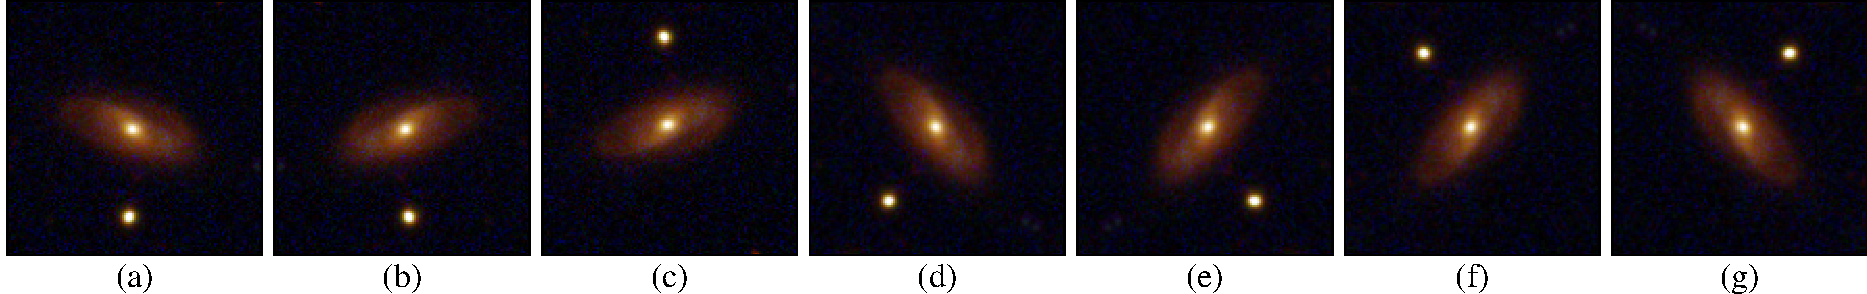
\includegraphics[width=\linewidth]{figures/dataaug.pdf}
  \legend{Exemplo do aumento artificial de dados em uma imagem original, mostrada no painel (a). Os painéis (b), (c), (d), (e), (f) e (g) contêm os resultados da eq. \eqref{eq:final-transformation} substituindo $M$ por diferentes combinações das transformações das eqs. \eqref{eq:aug-rot}, \eqref{eq:aug-h} e \eqref{eq:aug-v}. Em (b) $M = V$, em (c) $M = H$, em (d) $M = R(30\degree)$, em (e) $M = V R(30\degree)$, em (f) $M = H R(30\degree)$ e em (g) $M = H V R(30\degree)$.}
  \label{fig:dataaug}
\end{figure*}

Aumento artificial de dados \cite{Larry1996} é a aplicação de transformações afins nas imagens do conjunto de treinamento, por exemplo rotação, reflexão, translação e mudança de escala. As matrizes das eqs. \eqref{eq:aug-rot}, \eqref{eq:aug-h} e \eqref{eq:aug-v} definem as transformações usadas.


\begin{equation}\label{eq:aug-rot}
  R(\theta) =
  \begin{bmatrix}
    \cos(\theta) & -\sin(\theta) & 0 \\
    \sin(\theta) & \cos(\theta)  & 0 \\
    0            & 0             & 1
  \end{bmatrix}
\end{equation}


\begin{equation}\label{eq:aug-h}
  H =
  \begin{bmatrix}
    1 & 0  & 0 \\
    0 & -1 & 0 \\
    0 & 0  & 1
  \end{bmatrix}
\end{equation}


\begin{equation}\label{eq:aug-v}
  V =
  \begin{bmatrix}
    -1 & 0 & 0 \\
    0  & 1 & 0 \\
    0  & 0 & 1
  \end{bmatrix}
\end{equation}


onde $R(\theta)$ é a transformação rotação por um ângulo $\theta$,
$H$ é a transformação reflexão horizontal e $V$ é a transformação reflexão vertical, nas eqs. \eqref{eq:aug-rot}, \eqref{eq:aug-h} e \eqref{eq:aug-v}, respectivamente.

Seja $M$ a matriz das transformações combinadas, $(x, y)$ a coordenada do píxel da imagem original e $(x^*, y^*)$ a coordenada transformada do píxel, as transformações nas imagens são feitas remapeando as coordenadas dos píxeis originais aplicando uma combinação das matrizes das eqs. \eqref{eq:aug-rot}, \eqref{eq:aug-h} e \eqref{eq:aug-v} em cada píxel da imagem original usando a equação \eqref{eq:final-transformation}, onde $(t_x, t_y)$ é a coordenada do centro da imagem e as matrizes ao redor de $M$ são as matrizes translação. Isso é feito para que a transformação $M$ tenha o centro da imagem como ponto de simetria.

\begin{align} \label{eq:final-transformation}
  \begin{bmatrix}
    x^* \\
    y^* \\
    1
  \end{bmatrix}
  =
  \begin{bmatrix}
    1 & 0 & t_x \\
    0 & 1 & t_y \\
    0 & 0 & 1
  \end{bmatrix}
  \ M\
  \begin{bmatrix}
    1 & 0 & -t_x \\
    0 & 1 & -t_y \\
    0 & 0 & 1
  \end{bmatrix}
  \begin{bmatrix}
    x \\
    y \\
    1
  \end{bmatrix}
\end{align}

Além disso, ainda é aplicada uma interpolação bilinear como \emph{anti-aliasing} \cite{aliasing,bilinear}. Durante o treinamento da rede, novas imagens de entrada são geradas a cada época a partir da transformação das imagens originais. A Figura \ref{fig:dataaug} mostra a imagem original, no painel (a), e diversas transformações, nos demais painéis, aplicadas substituindo $M$ da equação \eqref{eq:final-transformation} por combinações (multiplicação matricial) das transformações das eqs. \eqref{eq:aug-rot}, \eqref{eq:aug-h} e \eqref{eq:aug-v}. Tais transformações não mudam a interpretação da classe da imagem original, pois o espaço visual é invariante a elas. Logo, o objetivo de aplicar estas transformações nas imagens de entrada da rede é deixar que o algorítmo infira tal invariância, criando, assim, uma ``noção'' do espaço visual, o que resulta no aumento do potencial de generalização da rede \cite{Simard2003,CholletBook}. Frequentemente são relatados bons resultados com o uso desta técnica \cite{EfficientNetEx01,EfficientNetEx02,CNNEx04}, principalmente quando existe grande similaridade entre as classes.






% \subsection{Preparação dos dados}
% \label{section:preparacao}

% O pré-processamento é a preparação das imagens para serem usadas pelo modelo, ou seja, é a transformação dos dados não processados em dados prontos para entrada na rede. Isso envolve representar as imagens por matrizes multidimensionais, onde cada elemento da matriz representa um pixel da imagem, e aplicar algumas transformações, especificadas a seguir.

% \subsubsection{Agrupamento das bandas para confecção das imagens RGB}

% Como as imagens do S-PLUS foram obtidas em 12 bandas fotométricas (listadas em \cite{splus}), para representá-las no sistema de cor RGB fizemos o seguinte mapeamento: em R colocamos as 4 bandas vermelhas r\_SDSS, i\_SDSS, J0861 e z, em G as bandas g\_SDSS J0515 e J0660 e em B as cinco bandas mais azuis u\_JAVA, J0373, J0395, J0410 e J0430 (as características destes filtros são dadas na Tabela 1 de \cite{splus}). Na combinação de bandas em cada canal, foi feita uma soma simples dos valores dos píxeis. Depois de reduzidas a três bandas, as imagens são usadas como entrada do programa Trilogy\cite{coe2012clash}\footnote{\url{https://www.stsci.edu/~dcoe/trilogy/Intro.html}}.

% \subsubsection{ImageNet}

% Como já mostrado em trabalhos anteriores, a inicialização dos pesos provenientes de uma rede pré-treinada usando a base de dados \emph{ImageNet}\footnote{\url{http://www.image-net.org/}} traz uma grande melhoria na precisão dos resultados da classificação. Essa base de dados possui milhões de imagens de objetos do cotidiano e já foi utilizada especificamente para a classificação de objetos astronômicos (veja por exemplo \cite{bom2021}), com excelentes resultados.

% O uso deste dataset para pré-treinamento respeitou o pré-processamento utilizado originalmente pelos autores de cada rede, este procedimento este foi crucial para garantir um fit competitivo, isto é, no \textit{benchmarking} original destas redes para os dados da \emph{ImageNet}. Para a rede VGG16 (Seção \ref{section:vgg}), a ordem das bandas foi trocada de RGB para BGR, e cada banda foi centrada em zero em relação à \emph{ImageNet}, sem escalonamento, ou seja, os píxeis de cada banda tiveram o valor da média da respectiva banda \emph{ImageNet} subraído. Para a rede InceptionResNetV2 (Seção \ref{section:inceptionresnetv2}), os píxeis de entrada foram escalonados entre -1 e 1 em relação a amostra de treino. Para a rede EfficientNet (Seção \ref{section:efficientnet}), os píxeis de entrada foram escalonados entre 0 e 1 em relação à amostra de treino. E, para a rede DenseNet (Seção \ref{section:densenet}), os píxeis de entrada foram escalonados entre 0 e 1 e cada banda foi padronizada em relação à \emph{ImageNet}, isto é, os píxeis de cada banda tiveram o valor da média subtraído e o resultado foi dividido pelo desvio padrão da distribuição da respectiva banda da \emph{ImageNet}.

% \begin{figure*}[!ht]
%   \centering
%   \includegraphics[width=\textwidth]{figures/arch.pdf}
%   \caption{Diagrama que descreve a arquitetura da rede. Da esquerda para a direita, as 12 imagens de cada banda são agrupadas em uma única imagem RGB (Seção \ref{section:preparacao}), que é a entrada dos classificadores indidviduais. Estes classificadores (Seção \ref{section:classificador}) têm a função de extrair características visuais da imagem e retornar a probabilidade de ser elíptica ou espiral. O meta-modelo (Seção \ref{section:meta-modelo}) tem a função de combinar as predições dos classificadores em uma única predição final mais robusta.}
%   \label{fig:arch}
% \end{figure*}






\subsection{Função de Custo}
\label{sec:modelo-loss}


\subsubsection{Distribuição Multinomial}
\label{sec:modelo-multi}

A distribuição multinomial \cite{distbook-multinomial} é uma generalização da distribuição binomial \cite{distbook-binomial} que descreve o comportamento de um experimento discreto onde cada tentativa resulta em um de $k$ possíveis resultados mutuamente exclusivos.

Supondo que um experimento é repetido $n$ vezes, e que a probabilidade de cada resultado específico $i$, para $i=1,2,\dots,k$, seja $p_i$, com $\sum_{i=1}^k p_i = 1$. A distribuição multinomial caracteriza a probabilidade conjunta de observar cada um dos $k$ resultados um número específico de vezes ($x_1, x_2,\dots, x_k$), onde $\sum_{i=1}^k x_i = n$. A função de probabilidade associada é definida pela eq. \eqref{eq:multinomial}, onde \( x_i \geq 0 \) representa a contagem de ocorrências para cada categoria \( i \).

\begin{equation}\label{eq:multinomial}
  P(X_1 = x_1, X_2 = x_2, \dots, X_k = x_k) = \frac{n!}{x_1! x_2! \cdots x_k!} \prod_{i=1}^k p_i^{x_i}
\end{equation}

A distribuição multinomial \cite{seber2015-multi} é amplamente utilizada em aplicações de aprendizado de máquina e estatística, como na modelagem da transmissão de Dengue \cite{wang2025}, na predição de cotação de mercado \cite{nevasalmi2020} e na análise de tráfego aéreo \cite{torres2023}. Uma de suas principais aplicações é em modelagem de eventos categóricos \cite{kibriya2004,luo2021}. Por exemplo, em tarefas de classificação multiclasse, onde o objetivo é prever a probabilidade de uma amostra pertencer a uma entre várias categorias, a distribuição multinomial é usada para modelar a saída do modelo. Um exemplo prático é o uso em algoritmos como o Naive Bayes Multinomial \cite{kalcheva2023,jiang2016}, amplamente empregado em problemas de classificação de texto \cite{odeh2022,kan2005}, como análise de sentimentos \cite{saravanan2023} e categorização de documentos. Neste contexto, as palavras em um documento são tratadas como eventos que seguem uma distribuição multinomial.

% Outra aplicação significativa é no modelamento de linguagens probabilísticas, como em modelos n-grama usados para processamento de linguagem natural (NLP). Nesses modelos, a distribuição multinomial é usada para representar a probabilidade de coocorrência de palavras em sequência. Além disso, na estimação de tópicos em conjuntos de documentos, como no algoritmo Latent Dirichlet Allocation (LDA), a distribuição multinomial é usada para modelar a distribuição de palavras em tópicos e tópicos em documentos.

% No campo de aprendizado profundo, a distribuição multinomial aparece em camadas de saída de redes neurais voltadas para classificação multiclasse, onde a função softmax é usada para transformar as saídas da rede em probabilidades que seguem uma distribuição multinomial. Esse uso é especialmente prevalente em problemas como reconhecimento de imagens e detecção de objetos.

% Por fim, a distribuição multinomial também desempenha um papel importante em amostragem e inferência estatística. Em métodos como amostragem Gibbs e Markov Chain Monte Carlo (MCMC), é comum gerar amostras a partir de distribuições multinomiais para explorar o espaço de parâmetros em modelos probabilísticos complexos.


\subsubsection{Distribuição de Dirichlet}
\label{sec:modelo-dir}

A distribuição Dirichlet \cite{distbook-dirichlet} é uma distribuição de probabilidade multivariada contínua definida no simplex \( k \)-dimensional, sendo uma generalização da distribuição Beta \cite{distbook-beta} para múltiplas dimensões. Ela é frequentemente utilizada para modelar distribuições de probabilidade sobre proporções, em que cada elemento do vetor de variáveis aleatórias representa uma fração de um todo e, portanto, suas somas totalizam 1.

Dada uma variável aleatória \( \vec{X} = (X_1, X_2, \dots, X_k) \) que segue uma distribuição Dirichlet com parâmetro de concentração \( \vec{\alpha} = (\alpha_1, \alpha_2, \dots, \alpha_k) \) para uma quantidade $k$ de categorias, a função de densidade de probabilidade é definida pela eq. \eqref{eq:dirichlet}, onde \( B(\vec{\alpha}) \) é a função beta multivariada, definida na eq. \eqref{eq:dirichlet-B}, e \( \Gamma(\cdot) \) representa a função gama \cite{distbook-gamma}. O parâmetro \( \alpha_i \) controla a concentração da probabilidade ao redor das categorias: valores maiores de \( \alpha_i \) indicam maior densidade de probabilidade associada à categoria correspondente.

\begin{equation}\label{eq:dirichlet}
  P(\vec{X} | \vec{\alpha}) = \frac{1}{B (\vec{\alpha})} \prod_{i=1}^k X_i^{\alpha_i - 1}
\end{equation}

\begin{equation}\label{eq:dirichlet-B}
  B(\vec{\alpha}) = \frac{\prod_{i=1}^k \Gamma(\alpha_i)}{\Gamma\left(\sum_{i=1}^k \alpha_i\right)}
\end{equation}


Em aprendizado de máquina, a distribuição Dirichlet possui aplicações importantes em problemas que envolvem modelagem de distribuições de probabilidade sobre categorias. Um exemplo clássico é na modelagem de misturas probabilísticas, como no algoritmo Latent Dirichlet Allocation (LDA; \citealp{lda}), amplamente utilizado para análise de tópicos em grandes corpora de texto \cite{jelodar2019}. No LDA, a distribuição Dirichlet é usada como uma distribuição a priori para representar a probabilidade de tópicos em documentos e a probabilidade de palavras em tópicos, fornecendo uma forma eficiente de capturar relações semânticas latentes \cite{canini2009}.

% Além disso, a distribuição Dirichlet é usada em inferência bayesiana, especialmente como conjugado da distribuição multinomial. Em tarefas como classificação multiclasse, a combinação da distribuição Dirichlet com a multinomial permite a atualização eficiente das probabilidades a priori para a modelagem de eventos categóricos. Esse mecanismo é essencial em algoritmos de aprendizado supervisionado que se baseiam em pressupostos probabilísticos, como o Naive Bayes Multinomial.

% Outro campo de aplicação da distribuição Dirichlet é o **aprendizado de misturas**, onde modelos como o Dirichlet Process Mixture Model (DPMM) usam essa distribuição para lidar com dados agrupados, mas com um número potencialmente infinito de clusters. Essa característica é particularmente útil em problemas não supervisionados, onde o número de classes ou clusters não é conhecido a priori.

% Na **simulação e geração de dados sintéticos**, a distribuição Dirichlet é frequentemente empregada para gerar distribuições de probabilidades em modelos de simulação. Por exemplo, em aprendizado por reforço, ela pode ser usada para modelar incertezas nas probabilidades de transição entre estados em ambientes estocásticos.

% Por fim, a distribuição Dirichlet também desempenha um papel em métodos de regularização. Em problemas de otimização envolvendo distribuições de probabilidades, ela pode ser usada para impor uma estrutura probabilística bem definida, evitando soluções degeneradas ou com concentração excessiva de probabilidades em poucas categorias.

% Em resumo, a distribuição Dirichlet é uma ferramenta central para modelar proporções e distribuições categóricas em múltiplas áreas do aprendizado de máquina, oferecendo uma base teórica sólida para lidar com problemas envolvendo incertezas e relações probabilísticas complexas.




\subsubsection{Distribuição Dirichlet-Multinomial}
\label{sec:modelo-dir-multi}

A distribuição Dirichlet-multinomial \cite{distbook-dirichlet} é uma distribuição de probabilidade discreta que combina as propriedades da distribuição multinomial (Seção \ref{sec:modelo-multi}) e da distribuição Dirichlet (Seção \ref{sec:modelo-dir}). Ela é usada para modelar processos em que as probabilidades das categorias em uma distribuição multinomial são, elas mesmas, amostras de uma distribuição Dirichlet. Isto é, a distribuição Dirichlet é usada como distribuição a priori para estimar os parâmetros da distribuição multinomial. Essa estrutura permite incorporar incertezas sobre as probabilidades subjacentes das categorias.

Formalmente, dado um vetor \( \vec{\theta} = (\theta_1, \theta_2, \dots, \theta_k) \) de probabilidades categóricas que segue uma distribuição Dirichlet com parâmetro \( \vec{\alpha} = (\alpha_1, \alpha_2, \dots, \alpha_k) \), e uma distribuição multinomial condicional sobre \( \vec{\theta} \), a probabilidade conjunta da distribuição Dirichlet-multinomial é expressa na eq. \eqref{eq:dirichlet-multinomial}, onde \( n = \sum_{i=1}^k x_i \) é o número total de experimentos, e \( x_i \) representa o número de ocorrências da \( i \)-ésima categoria.

\begin{equation}\label{eq:dirichlet-multinomial}
  P(X_1 = x_1, X_2 = x_2, \dots, X_k = x_k) = \frac{\Gamma\left(\sum_{i=1}^k \alpha_i\right)}{\Gamma\left(\sum_{i=1}^k \alpha_i + n\right)} \prod_{i=1}^k \frac{\Gamma(x_i + \alpha_i)}{\Gamma(\alpha_i) \, x_i!}
\end{equation}




\subsubsection{Função de Custo e Função de Perda}
\label{sec:modelo-loss-cost}

A função de perda (\emph{loss function}) e a função de custo (\emph{cost function}) têm papéis relacionados, mas distintos. A primeira avalia o erro do modelo em uma única amostra, medindo a discrepância entre a predição do modelo e o valor esperado. Já a segunda, é uma agregação da primeira, geralmente calculada como a média ou soma das perdas sobre todo o conjunto de treinamento, representando o desempenho global do modelo. %Isto é, enquanto a loss function opera em nível de exemplo individual, a cost function fornece uma visão geral para otimizar o modelo durante o treinamento.

% A escolha da função de perda possui impacto direto na capacidade preditiva do modelo. Por isso, escolhemos uma função de custo

% As informações morfológicas sobre as galáxias são obtidas pelo projeto GalaxyZoo, que consistem nos votos de voluntários para diversas perguntas sobre suas características visuais, como a orientação espacial, a presença de bojo, a quantidade de braços espirais, etc. Então, considerando a origem dos dados, a distribuição Dirichlet-multinomial (Seção \ref{sec:modelo-dir-multi}) foi escolhida como função de custo.

A função de perda de uma pergunta $q$ é calculada a partir da distribuição Dirichlet-Multinomial, conforme a eq. \eqref{eq:loss}.

\begin{equation}\label{eq:loss}
  \mathcal{L}_q = \int\text{Multi}(\vec{k}|\vec{\rho}, N) \text{Dirichlet}(\vec{\rho}|\vec{\alpha})d\vec{\rho}
\end{equation}

Já o valor da perda de um exemplo é a soma das perdas de cada questão $q$, conforme a eq. \eqref{eq:log_loss}.

\begin{equation}\label{eq:log_loss}
  \log \mathcal{L} = \sum_q \mathcal{L}_q(\vec{k_q}, N_q, \vec{f_q^w})
\end{equation}

Existem duas formas recorrentes de agregar as perdas dos exemplos para calcular o custo total do modelo: calcular a soma  ou a média. Nesse trabalho, a função de custo é definda como a soma de todas as perdas de cada exemplo do conjunto de dados, conforme eq. \eqref{eq:cost}.

\begin{equation}\label{eq:cost}
  J = \sum_i \log \mathcal{L}_i
\end{equation}


% ### Propriedades e Intuição
% A distribuição Dirichlet-multinomial é uma extensão prática da distribuição multinomial porque incorpora variabilidade adicional na estimativa das probabilidades \( \boldsymbol{\theta} \). Isso a torna ideal para modelar dados categóricos onde há incerteza ou variabilidade na distribuição subjacente. Como tal, ela é frequentemente descrita como uma multinomial com parâmetros aleatórios seguindo uma Dirichlet.

% ### Aplicações em Aprendizado de Máquina
% No campo de aprendizado de máquina, a distribuição Dirichlet-multinomial possui aplicações significativas em **modelagem probabilística** e **inferência bayesiana**. Uma de suas utilizações mais comuns é na modelagem de fenômenos categóricos em que a frequência das categorias varia entre diferentes conjuntos de dados ou instâncias.

% #### 1. **Latent Dirichlet Allocation (LDA)**
% Na análise de tópicos, a Dirichlet-multinomial é usada para modelar a distribuição das palavras em documentos. Cada documento é tratado como uma realização de uma multinomial, cujas probabilidades de categorias (palavras) são amostras de uma Dirichlet. Essa abordagem permite capturar as variações de distribuição de palavras entre tópicos, sendo central para algoritmos como o **Latent Dirichlet Allocation (LDA)**, amplamente utilizado em **processamento de linguagem natural**.

% #### 2. **Inferência Bayesiana em Classificação Multiclasse**
% A Dirichlet-multinomial é o modelo conjugado da distribuição multinomial em inferência bayesiana. Em problemas de **classificação multiclasse**, ela é usada para modelar a incerteza nas estimativas das probabilidades das classes, particularmente em cenários de aprendizado supervisionado onde os dados de treinamento são limitados.

% #### 3. **Modelagem de Contagens e Variabilidade**
% Problemas que envolvem dados de contagem, como análise de redes sociais, preferências de usuários ou frequências de eventos em sistemas distribuídos, frequentemente apresentam superdispersão (variância maior que a média). A Dirichlet-multinomial é adequada para modelar essa superdispersão, fornecendo uma alternativa robusta à multinomial tradicional.

% #### 4. **Misturas de Modelos e Clusterização**
% Na clusterização, especialmente em métodos baseados em misturas, como o **Dirichlet Process Mixture Models (DPMM)**, a Dirichlet-multinomial pode ser usada para modelar distribuições de contagens em diferentes clusters. Esse uso é especialmente relevante em problemas de agrupamento não supervisionado.

% #### 5. **Geração de Dados Sintéticos**
% A distribuição Dirichlet-multinomial também é amplamente utilizada para gerar dados categóricos sintéticos que incorporam incertezas ou variabilidades realistas, sendo valiosa em experimentos controlados e validações de algoritmos.

% ### Conclusão
% A distribuição Dirichlet-multinomial é uma ferramenta poderosa para modelar processos categóricos que exibem variabilidade nas probabilidades subjacentes. Sua capacidade de capturar incertezas intrínsecas torna-a essencial em uma ampla gama de aplicações, especialmente na modelagem de tópicos, inferência bayesiana e análise de dados de contagem. No aprendizado de máquina, ela desempenha um papel central ao lidar com problemas onde a variabilidade das distribuições subjacentes é uma característica fundamental dos dados.




\subsection{Hiperparâmetros}
\label{sec:modelo-hp}

Nesta seção descrevemos as definições dos principais conceitos, no contexto de deep learning, que serão úteis para o entendimento dos métodos aqui utilizados. A função de ativação, função de custo, o otimizador, o learning rate, o número de épocas, além do número de camadas dos modelos, são importantes parâmetros responsáveis pela contrução do modelo definido a seguir.

\begin{description}
  \item[Função de ativação] \hfill \\
        A função de ativação é responsável por adicionar não-linearidade à rede. Sem ela, a saída de uma camada seria apenas uma transformação linear dos dados de entrada e a rede não seria beneficiada pelo empilhamento de diversas camadas lineares, pois isso não aumentaria o espaço de hipóteses. Logo, a função de ativação viabiliza representações mais complexas da rede, uma vez que define a complexidade de um modelo e, consequentemente, sua capacidade de generalização \cite{CholletBook}. Neste trabalho, a função $\textrm{ReLU}(x) := \textrm{max}(0, x)$ é usada nas camadas densas dos classificadores, a equação tangente hiperbólica é usada nas camadas densas do meta-modelo e a função Softmax \cite{Bridle1990} foi usada na última camada, tanto dos classificadores quanto do meta-modelo.

  \item[Otimizador] \hfill \\
        O otimizador é um algorítmo iterativo com objetivo de minimizar a função de custo. Uma escolha típica é o método de gradiente descente e suas demais variações. Este tipo de algoritmo tem um parâmetro livre relacionado ao passo da iteração conhecido como taxa de aprendizado ou \textit{learning rate}. Neste trabalho foram testados diversos algoritmos considerados como estado-da-arte dos otimizadores como Adam \cite{Adam}, NAdam \cite{NAdam}, RAdam \cite{RAdam} e RMSprop \cite{RMSprop}.

  \item[Número de Épocas] \hfill \\
        O Número de épocas se referem a quantidade de vezes que o dataset de treino foi utilizado completamente no processo de otimização iterativa da função de custo. Um número de épocas adequado é necessário para que a função de custo seja minimizada.

  \item[Tamanho do Batch] \hfill \\
        O processo de otimização acontece em batches, cada iteração para minimizar a função custo é realizada com um número fixo de amostras, quando todas as amostras de treino são utilizadas se completa uma época.

  \item[Unidades de neurônios na última camada]
        \hfill \\
        A última camada da rede antes da camada de saída é responsável por condensar toda a informação extraída da rede para o processo de classificação final. Por esta razão, a quantidade de neurônios nessa camada pode ser particularmente sensível para a performance da rede. Neste trabalho utilizamos diferentes valores de neurônios para encontrar a quantidade que pode gerar a melhor performance.

  \item[Dropout]
        \hfill \\
        \emph{Dropout} \cite{dropout} é uma técnica de regularização muito utilizada em redes neurais por seu bom desempenho e baixo custo computacional. Aplicar esta regularização em uma camada consiste em eliminar aleatoriamente uma taxa dos neurônios de saída desta camada durante o treinamento, sendo geralmente escolhido um valor entre 0.2 e 0.5 para esta taxa \cite{CholletBook}.
\end{description}












\subsection{Arquitetura de Rede Neural}
\label{sec:arch}

\subsubsection{Visual Geometry Group Networks}
\label{sec:vgg}
A família de arquiteturas Visual Geometry Group Networks (VGGNets) \cite{VGG16} foi criada durante a competição de classificação de imagens \textit{Large Scale Visual Recognition Challenge} \cite{ILSVRC15}. Ela se destaca por estar entre as primeiras redes a adotar, com sucesso, o escalamento em profundidade (quantidade de camadas) para aumentar o desempenho na classificação de imagens usando redes convolucionais. Neste trabalho, consideramos a arquitetura VGG16, que já foi usada em diversas tarefas de classificação, como a classificação de software malicioso \cite{VGG16Ex01}, de plantas \cite{VGG16Ex02} e de tumores cerebrais \cite{VGG16Ex03}.

\subsubsection{InceptionResNetV2}
\label{sec:inceptionresnetv2}
A arquitetura InceptionResNetV2 \cite{InceptionResNetv2} usa os blocos Inception, que são convoluções fatorizadas, introduzidos em \cite{Inception}, motivada pela construção de redes mais profundas com um menor custo computacional e menor overfitting, com a adição de conexões residuais \cite{ResNet} motivada pelo problema de dissipação do Gradiente (\textit{vanishing gradients}). Isso permite treinar redes profundas com maior acurácia e mais rápido. Esta arquitetura já foi usada, por exemplo, para classificação de imagens de satélite \cite{InceptionResNetV2Ex01}, de ultrasonografia \cite{InceptionResNetV2Ex02} e de células cancerígenas \cite{InceptionResNetV2Ex03}.

\subsubsection{EfficientNet}
\label{sec:efficientnet}
A arquitetura EfficientNet \cite{EfficientNet} foi desenvolvida como uma resposta à questão de como escalar modelos de convolução. Foram considerados três diferentes aspectos: profundidade, largura e resolução da imagem de entrada. Em vez de dimensionar cada aspecto manualmente, o modelo implementa um escalonamento composto que equilibra os aspectos para obter melhor desempenho, com isso a rede consegue uma alta acurácia usando muito menos parâmtros e operações de ponto flutuante por segundo (\emph{FLOPS}). Esta rede já foi usada na classificação de doenças em vegetais \cite{EfficientNetEx03}, eletrocardiogramas \cite{EfficientNetEx01} e cristalização de proteínas \cite{EfficientNetEx02}.

\subsubsection{DenseNet}
\label{sec:densenet}
A rede DenseNet \cite{DenseNet} também usa conexões residuais que conectam cada camada a todas as outras camadas seguintes, o que reduz ainda mais o número de parâmetros na rede sem perda significativa da precisão. O uso desta rede incluem predição do mapa de contato de proteínas \cite{DenseNetEx02}, classificação de músicas \cite{DenseNetEx05}, câncer de mama \cite{DenseNetEx01} e esclerose múltipla \cite{DenseNetEx03}.


\subsubsection{Escolha da Arquitetura}
\label{sec:escolha-arch}
Todas as arquiteturas convolucionais mencionadas nessa seção foram testadas e a arquitetura que teve melhor desempenho na predição dos votos dos voluntários foi escolhida. O processo de treinamento e avaliação está descrito na seção seguinte.



\subsection{Treinamento}
\label{sec:modelo-treinamento}

O treinamento de modelos de aprendizado profundo é um processo complexo que envolve a escolha de uma arquitetura adequada e a definição de hiperparâmetros que otimizem o desempenho do modelo em um conjunto de dados específico. A técnica de treinamento automatizado (AutoML; \citealp{automl}), mostrada na Fig. \ref{fig:treinamento}, facilita esse processo de seleção de hiperparâmetros e configurações de treinamento. Neste trabalho, foi utilizada uma abordagem que se mostrou eficaz nesse contexto: os algoritmos Multi-Objective Tree-structured Parzen Estimator (MOTPE; \citealp{motpe}) e HyperBand (HB; \citealp{hyperband}), disponíveis na biblioteca Optuna\footnote{\url{https://optuna.org}} \cite{optuna}, para a otimização de múltiplos objetivos simultaneamente.

\begin{figure}[!ht]
  \centering
  \caption{Treinamento do modelo}
  \label{fig:treinamento}
  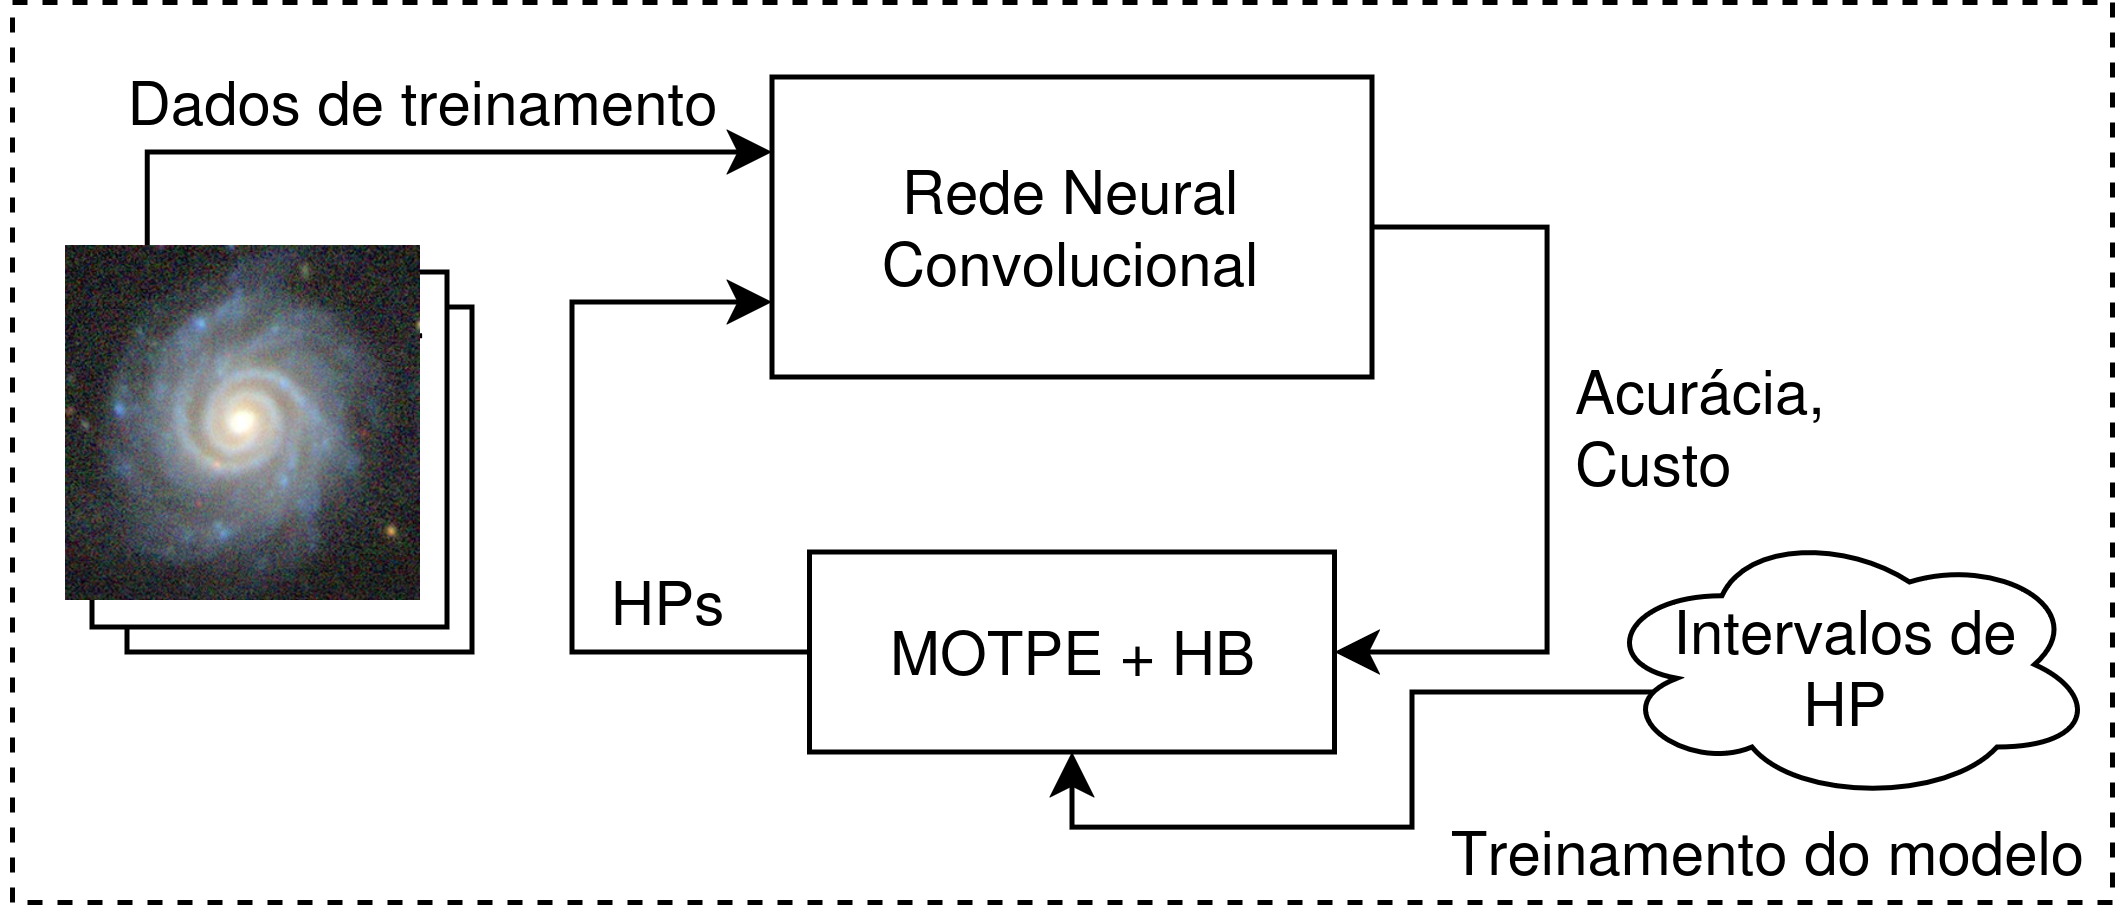
\includegraphics[width=\linewidth]{figures/treinamento.png}
\end{figure}

O treinamento com AutoML utilizando o MOTPE envolve diversas etapas estruturadas, desde a configuração inicial do espaço de busca dos hiperparâmetros até a avaliação iterativa dos modelos. A seguir, descrevem-se as principais etapas do processo:

\begin{enumerate}
  \item \textbf{Definição do Espaço de Busca dos Hiperparâmetros:}
        Inicialmente, define-se um espaço de busca para os hiperparâmetros do modelo, que pode incluir a taxa de aprendizado, número de camadas, número de neurônios por camada, taxas de dropout, tipos de ativação, otimizadores, entre outros. Para cada hiperparâmetro, especificam-se limites, distribuições ou valores discretos que serão explorados pelo algoritmo.

  \item \textbf{Criação da Função de Objetivo:}
        A função de objetivo é o núcleo do processo de otimização. Ela recebe uma configuração de hiperparâmetros como entrada, treina e avalia o modelo utilizando essa configuração, e retorna uma ou mais métricas de desempenho que serão otimizadas. No caso do MOTPE, que é multiobjetivo, é possível considerar métricas conflitantes, como minimizar o erro de validação enquanto reduz o tempo de treinamento.

  \item \textbf{Treinamento Iterativo com Amostragem Bayesiana:}
        O MOTPE utiliza um modelo probabilístico para guiar a busca por configurações promissoras. Ele avalia iterativamente as combinações de hiperparâmetros, ajustando o modelo probabilístico com base nos resultados obtidos em iterações anteriores. Isso permite uma exploração mais eficiente do espaço de busca, concentrando-se em áreas com maior probabilidade de melhorar o desempenho.

  \item \textbf{Validação e Regularização:}
        Cada configuração de hiperparâmetros é validada em um conjunto de validação separado para garantir que o modelo não esteja superajustando os dados de treinamento. Além disso, o uso de técnicas como early stopping e regularização (L2 ou dropout) é integrado ao treinamento para evitar overfitting.

  \item \textbf{Seleção do Melhor Modelo:}
        Após um número predefinido de iterações ou ao atingir um critério de parada, o AutoML seleciona a configuração de hiperparâmetros que apresenta o melhor desempenho médio em relação às métricas otimizadas. No caso de otimização multiobjetivo, a solução é escolhida com base no conceito de fronteira de Pareto.
\end{enumerate}

A Tabela \ref{tab:hps} sumariza os hiperparâmetros otimizados pelo MOTPE. Nela são mostrados os intervalos de busca para cada hiperparâmetro, bem como a distribuição utilizada para cada um deles.


\begin{table}[!ht]
  \centering
  \caption{Intervalos de busca dos hiperparâmetros otimizados com o MOTPE}
  \label{tab:hps}
  \begin{tabular}{lll}
    \toprule
    Hiperparâmetro            & Distribuição     & Intervalo de Busca              \\
    \midrule
    Arquitetura               & Categórica       & \{VGG, IRV2, EffNet, DenseNet\} \\
    Taxa de aprendizado       & Log-Uniforme     & $[10^{-5}, 10^{-1}]$            \\
    Número de camadas ocultas & Int-Uniforme     & $[0, 5]$                        \\
    Neurônios por camada      & Int-Uniforme     & $[32, 512]$                     \\
    Taxa de dropout           & Uniforme         & $[0.1, 0.5]$                    \\
    Otimizador                & Categórica       & \{Adam, NAdam, SGD, RMSprop\}   \\
    Batch size                & Int-Log-Uniforme & $[16, 256]$                     \\
    Peso da regularização L2  & Log-Uniforme     & $[10^{-5}, 10^{-2}]$            \\
    Função de ativação        & Categórica       & \{ReLU, Leaky ReLU, ELU\}       \\
    \bottomrule
  \end{tabular}
\end{table}




\subsection{Métricas de Avaliação da Predição dos Votos}
\label{sec:metricas-votos}

As métricas aqui utilizadas baseiam-se no erro ou acerto na associação dos objetos às classes pelo modelo. Para relacionar a probabilidade calculada pelo modelo à classe, é definido um limiar de discriminação, que é a probabilidade mínima para que um exemplar pertença à uma classe. Para o cálculo das métricas, foi considerado um de limiar de 0.5.

\subsubsection{Matriz de Confusão}
\label{sec:metricas-confusao}

A matriz de confusão consiste em um modelo tabular que cruza métricas de predição e referência, sendo comumente usada para avaliar a qualidade preditiva de modelos de aprendizagem de máquina. A Tabela \ref{tab:cm} mostra um esquema desta matriz para o caso de classificação binária (apenas duas classes). A análise para mais classes pode ser feita isolando uma classe positiva por vez e reduzindo o problema a multiplas classificações binárias.

\begin{table}[!ht]
  \centering
  \caption{Estrutura da matriz de confusão para classificação binária}
  \label{tab:cm}
  \begin{tabular}{lll}
    \toprule
    {}                          & \multicolumn{2}{c}{Predição}                            \\
    \midrule
    \multirow{2}{*}{Verdadeiro} & Verdadeiro Positivo (VP)     & Falso Negativo (FN)      \\
    {}                          & Falso Positivo (FP)          & Verdadeiro Negativo (VN) \\
    \bottomrule
  \end{tabular}
\end{table}

A seguir, são definidas cada uma das métricas usadas para montar a matriz de confusão.

\begin{itemize}
  \item Verdadeiro Positivo (VP): O modelo prevê uma instância verdadeira corretamente
  \item Verdadeiro Negativo (VN): O modelo prevê uma instância negativa corretamente
  \item Falso Positivo (FP): O modelo prevê uma instância positiva, mas, na verdade, é negativa. Este é o erro tipo I, que consiste em rejeitar a hipótese nula quando ela é verdadeira.
  \item Falso Negativo (FN): O modelo prevê uma instância negativa, mas, na verdade, é positiva. Este é o erro tipo II, em estatística, que consiste na falha em rejeitar a hipótese nula quando ela é falsa.
\end{itemize}



\subsubsection{Acurácia}
\label{sec:metricas-acc}

A acurácia é uma métrica que mede a proporção de predições corretas em relação ao total de instâncias avaliadas. Ela é definida como indicado na eq. \ref{eq:acc}.

\begin{equation}\label{eq:acc}
  \text{Acurácia} = \frac{\text{VP} + \text{VN}}{\text{VP} + \text{VN} + \text{FP} + \text{FN}}
\end{equation}



\subsubsection{Precisão}
\label{sec:metricas-precisao}

A precisão avalia a proporção de exemplos classificados como positivos que são realmente positivos, conforme a eq. \eqref{eq:precisao}, sendo particularmente importante em cenários onde o custo de falsos positivos é alto.

\begin{equation}\label{eq:precisao}
  \text{Precisão} = \frac{\text{VP}}{\text{VP} + \text{FP}}.
\end{equation}




\subsubsection{Revocação}
\label{sec:metricas-revocacao}

A revocação, também conhecida como sensibilidade ou taxa de verdadeiros positivos, mede a capacidade do modelo de identificar corretamente os exemplos positivos, conforme a eq. \eqref{eq:recall}, sendo principalmente útil em contextos onde a identificação de todos os exemplos positivos é crucial

\begin{equation}\label{eq:recall}
  \text{Revocação} = \frac{\text{VP}}{\text{VP} + \text{FN}}.
\end{equation}




\subsubsection{F1-Score}
\label{sec:metricas-f1}

O F1-score é a média harmônica entre precisão e revocação, sendo usado como uma métrica de equilíbrio entre essas duas dimensões, conforme a eq. \eqref{eq:f1}. Esta métrica é útil quando há uma compensação entre precisão e revocação, como em cenários com classes desbalanceadas, pois fornece uma medida única que leva em conta ambos os aspectos. Valores de \( F1 \) próximos de 1 indicam que o modelo apresenta um bom equilíbrio entre os dois fatores.

\begin{equation}\label{eq:f1}
  F1 = 2 \cdot \frac{\text{Precisão} \cdot \text{Revocação}}{\text{Precisão} + \text{Revocação}}
\end{equation}









\section{Avaliação do Modelo no Conjunto de Teste}
\label{sec:res-teste}

A análise quantitativa das métricas de desempenho no conjunto de teste é fundamental para avaliar a capacidade preditiva e de generalização de um modelo de aprendizado profundo. A Tabela \ref{tab:test-metrics} sumariza as métricas de acurácia (Seção \ref{sec:metricas-acc}), precisão (Seção \ref{sec:metricas-precisao}), revocação (Seção \ref{sec:metricas-revocacao}) e F1-score (Seção \ref{sec:metricas-f1}) para várias perguntas do GalaxyZoo.

\begin{table}[!ht]
  \centering
  \caption{Avaliação do modelo no conjunto de teste}
  \label{tab:test-metrics}
  \begin{tabular}{lcccc}
    \toprule
    Questão            & Acurácia & Precisão & Revocação & F1       \\
    \midrule
    Spiral winding     & 0.833771 & 0.714138 & 0.717103  & 0.715594 \\
    Bar                & 0.890751 & 0.715289 & 0.780659  & 0.742811 \\
    Edge on bulge      & 0.943199 & 0.817953 & 0.895207  & 0.851695 \\
    Disk edge on       & 0.973585 & 0.969010 & 0.970718  & 0.969856 \\
    Smooth or featured & 0.974996 & -        & -         & -        \\
    Has spiral arms    & 0.942789 & 0.898665 & 0.859011  & 0.877276 \\
    Galaxy Symetrical  & 0.980000 & 0.973438 & 0.966997  & 0.970173 \\
    Clumpy appearence  & 0.962085 & 0.956045 & 0.958264  & 0.957141 \\
    How rounded        & 0.952254 & 0.919239 & 0.927339  & 0.923121 \\
    Merging            & 0.981400 & 0.666607 & 0.771892  & 0.703503 \\
    Bulge size         & 0.931864 & 0.683324 & 0.734342  & 0.701055 \\
    Spiral arms count  & 0.954545 & 0.684281 & 0.758884  & 0.716117 \\
    \bottomrule
  \end{tabular}
\end{table}

Para dar continuidade na avaliação quantitativa no conjunto de teste, a seguir, são mostradas as matrizes de confusão (Seção \ref{sec:metricas-confusao}) para questão da Tabela \ref{tab:test-metrics}.


\begin{figure}[!ht]
  \centering
  \caption{Matrizes de confusão para cada questão no conjunto de teste}
  \label{fig:cm_1}
  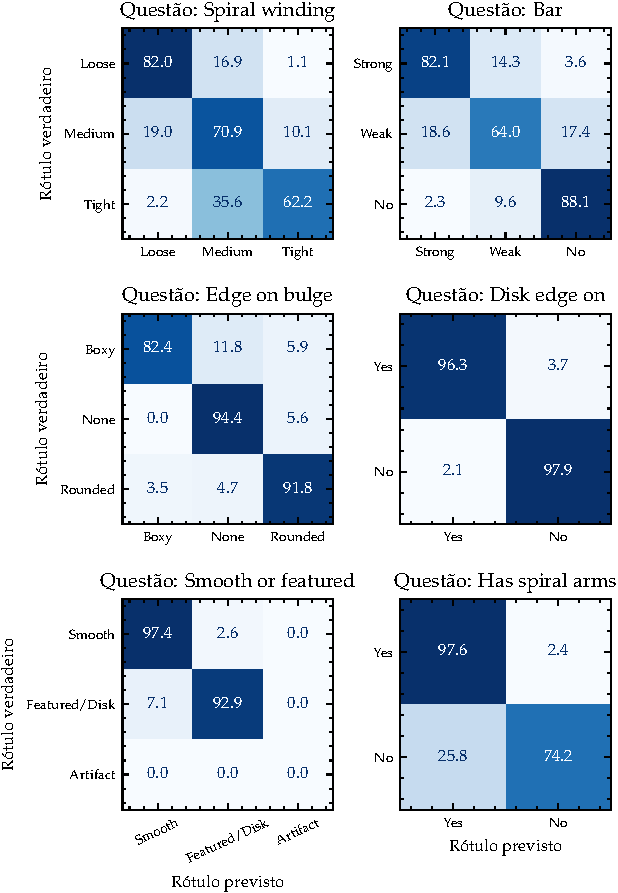
\includegraphics[width=\linewidth]{notebooks/plots/cm_1.pdf}
\end{figure}

\begin{figure}[!ht]
  \centering
  \caption{Matrizes de confusão para cada questão no conjunto de teste (continuação)}
  \label{fig:cm_2}
  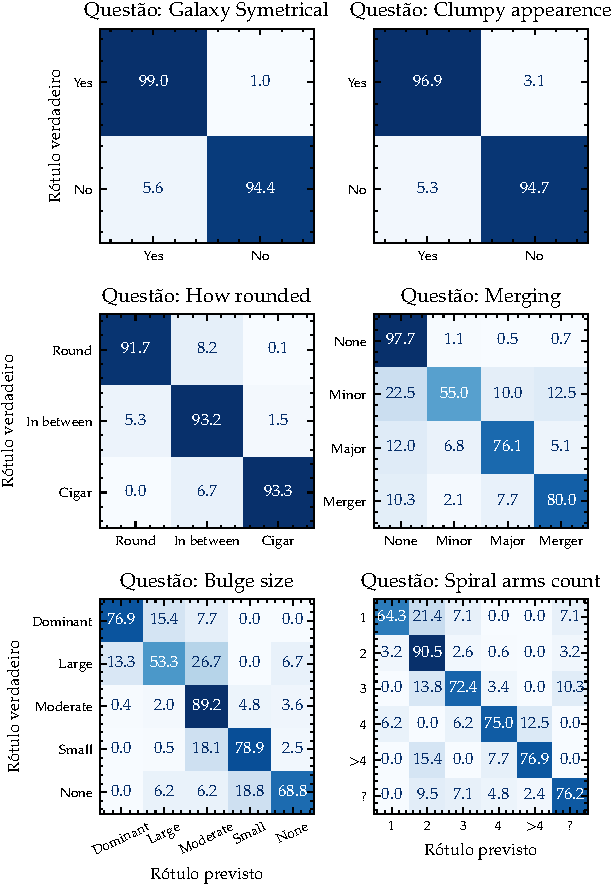
\includegraphics[width=\linewidth]{notebooks/plots/cm_2.pdf}
\end{figure}


Os velores mostrados na Tabela \ref{tab:test-metrics} e nas Figs. \ref{fig:cm_1} e \ref{fig:cm_2} mostram a eficiência do modelo em identificar as características morfológicas das galáxias. Essa análise evidencia que o modelo não apenas possui bom desempenho em dados de treinamento, mas também é capaz de generalizar para novos conjuntos de dados, aspecto crucial para aplicações científicas confiáveis.

\chaptersep
